\documentclass[../main.tex]{subfiles}

\graphicspath{{\subfix{../images/}}}

\begin{document}


\clearpage
\thispagestyle{empty}
\vspace*{7cm}
\section{Operational amplifiers}
\vspace*{1.5cm}

\subsection{Introductory analysis}

In this preliminary sections we will now go over the basic of what is an operational amplifier and its working principles.
Here below in \autoref{figopamp} we can see the diagram of the operational amplifier that wi will be using as a building block in the following sections.


\begin{figure}[h!]
\begin{center}

\begin{tikzpicture}[transform shape]
	\node[op amp, yscale=-1] at (9.083, 6.961){};
	\draw (9, 7.5) -| (9, 8.25);
	\draw (9, 6.422) -| (9, 5.75);
	\draw (8.875, 8.25) -- (9.125, 8.25);
	\draw (8.875, 5.75) -- (9.125, 5.75);
	\node[shape=rectangle, minimum width=0.215cm, minimum height=0.215cm] at (8.875, 8.625){} node[anchor=center, align=center, text width=-0.173cm, inner sep=6pt] at (8.875, 8.625){$V_{cc}$};
	\node[shape=rectangle, minimum width=0.215cm, minimum height=0.215cm] at (8.875, 5.375){} node[anchor=center, align=center, text width=-0.173cm, inner sep=6pt] at (8.875, 5.375){$V_{ee}$};
	\draw (7.625, 7.875) to[open, v_<=$v_d$, voltage/bump b=0.6] (7.625, 6);
	\node[ocirc](N1) at (10.273, 6.961){} node[anchor=west] at (N1.text){$V_{out}$};
	\node[ocirc] at (7.893, 6.471){};
	\node[ocirc] at (7.893, 7.451){};
\end{tikzpicture}

\caption{Circuit diagram of the operational amplifier}
\label{figopamp}	
\end{center}	
\end{figure}


The simplest approach to studying circuits based on operational amplifiers involves using a \textit{"black-box"} model (which does not specify the internal structure of the device in question). 

The most commonly used representation for the operational amplifier is that of a \textit{"triangle"} which is equipped with two input terminals, two power supply terminals (often omitted in circuits), and one output terminal; the input terminals, marked with the symbols "$+$" and "$-$" (also referred to as \textit{"non-inverting input"} and \textit{"inverting input"} respectively), are the inputs for the signals that the operational amplifier is intended to amplify; the power supply terminals, as the name suggests, are intended to bias and supply power to the circuit contained within the operational amplifier, in order to ensure its proper operation.\\

As we can see the power terminal are named $V_{cc}$ and $V_{ee}$ representing the high and low side of the power supply powering the amplifier that internally is composed of BJT transistor. The naming would be different ($V_{dd}$ and $V_{ss}$) in the case of the usage of MOSFET technology.\\

Further more we can see that on the output connection we can find $V_{out}$ which is obtain by knowing the gain of the amplifier and the differential voltage $v_d$ applied to the inputs terminals. 


\subsubsection{Differential amplifier}

Given now a preliminary introduction we can further more analyze this componente following its behaviors that is the ability to amplify the difference, voltage drop $v_d$, across its two input terminal following this relations from:

\begin{equation}
	V_{out} = A_d \cdot v_d
\end{equation}

As we can see the operational amplifier can amplify by a certain factor $A_d$, called open-loop differential gain, the difference $v_d$ called differential voltage, that is presented across its input terminal. It is now easy to understand why we get the term \textit{"differential"} amplifier.\\

Given now this additional piece of information we can start to make some assumptions on the value and the relative meaning of the quantities we have just described.\\

The open-loop differential gain $A_d$ (we will see why open-loop) is a very large number with an order of magnitude of around $10^5$ to $10^6$ that tells you how much will the amplifier amplify the differential voltage $v_d$.\\

Since the output voltage $V_{out}$ cannot be greater than the voltages that power the amplifier ($V_{cc}$ and $V_{ee}$) having a very big differential open-loop gain can be a problem since even a small differential input will quickly results in the output reaching the power supply limit and \textit{"saturating"} the output.\\

We can represent this situation with a graph as seen in \autoref{saturations}\\

\begin{figure}[h!]
\begin{center}

\begin{tikzpicture}[transform shape, scale = 0.8]
	\draw[-latex] (9, 3) -- (9, 11);
	\draw[-latex] (4, 7) -- (14, 7);
	\path[draw={rgb,255:red,0;green,86;blue,214}, line width=0.8pt] (6, 4) -- (12, 10);
	\path[draw={rgb,255:red,0;green,86;blue,214}, line width=0.8pt] (12, 10) -- (13, 10);
	\path[draw={rgb,255:red,0;green,86;blue,214}, line width=0.8pt] (6, 4) -- (5, 4);
	\path[draw={rgb,255:red,0;green,86;blue,214}, line width=0.8pt, dash pattern={on 3.2pt off 6.4pt}] (13, 10) -- (14, 10);
	\path[draw={rgb,255:red,0;green,86;blue,214}, line width=0.8pt, dash pattern={on 3.2pt off 6.4pt}] (4, 4) -- (5, 4);
	\draw[dash pattern={on 1.6pt off 3.2pt}] (6, 4) -- (9, 4);
	\draw[dash pattern={on 1.6pt off 3.2pt}] (9, 10) -- (12, 10);
	\node[shape=rectangle, minimum width=0.34cm, minimum height=0.34cm] at (14.437, 7){} node[anchor=center, align=center, text width=-0.048cm, inner sep=6pt] at (14.437, 7){$v_d$};
	\node[shape=rectangle, minimum width=0.34cm, minimum height=0.34cm] at (9, 11.375){} node[anchor=center, align=center, text width=-0.048cm, inner sep=6pt] at (9, 11.375){$V_{out}$};
	\node[shape=rectangle, minimum width=0.34cm, minimum height=0.34cm] at (8.438, 10){} node[anchor=center, align=center, text width=-0.048cm, inner sep=6pt] at (8.438, 10){$V_{cc}$};
	\node[shape=rectangle, minimum width=0.34cm, minimum height=0.34cm] at (9.438, 4){} node[anchor=center, align=center, text width=-0.048cm, inner sep=6pt] at (9.438, 4){$V_{ee}$};
	\draw[dash pattern={on 1.6pt off 3.2pt}] (6, 8) -- (6, 4);
	\draw[dash pattern={on 1.6pt off 3.2pt}] (12, 10) -- (12, 8);
	\draw[-latex] (9, 8) -- (12, 8);
	\draw[-latex] (9, 8) -- (6, 8);
	\node[shape=rectangle, minimum width=1.09cm, minimum height=0.465cm] at (7.938, 8.375){} node[anchor=center, align=center, text width=0.702cm, inner sep=6pt] at (7.938, 8.375){$\Delta v_{d_{linear}}$};
\end{tikzpicture}
	
\caption{Linear and saturation zones of an operational amplifier}	
\label{saturations}	
\end{center}	
\end{figure}

As we can see we can evaluate a region of linearity where there is no saturation that we call $\Delta v_{d_{linear}}$. Assuming now $A_d$ of $10^5$ and $V_{cc}$ = + 15 V and $V_{ee}$ = - 15 V we can calculate the linearity region.

\begin{equation}
	\Delta v_{d_{linear}} = \frac{15 - (-15)}{10^5} = \frac{30}{10^5} = 300\; \mu \unit{V}
\end{equation}

As we can see, from the data we calculated, the linearity region, is extremely small and any differential voltage bigger that 300 $\mu$V applied will result in the output reaching the power supply limit.\\

Before moving on we want to clarify that in the saturation region the output signal will reach the power supply limit only if the operational amplifier is a rail-to-rail one, if it is not the output voltage will be slightly lower than the limit.

\subsubsection{Ideal operational amplifiers}


After introducing the diagram, the basic working principle and seeing a pretty big limit in the operation amplifier (small linear region) we can move on to analyze the specification of the ideal operation amplifier with the end goal of removing each ideal assumption that we made to extrapolate a non-ideal model that we can use.\\

These equations are fundamental to the study of a general circuit containing one (or more) operational amplifiers.\\ 

Since the op-amp has a gain tending to infinity, it can be inferred that, in order to have a finite output that is, so that the result of the product of the differential voltage $v_d$ (voltage between the "$+$" and "$-$" terminals) and the op-amp’s differential gain $A_d$ is finite $v_d$ must tend to 0.

Consequently, in the ideal operational amplifier, the voltage drop across the terminals is nearly zero and the input current is nearly zero, regardless of the differential resistance present between the input terminals. 

We can non express what we have just said via some useful formulas:

\begin{equation}
	V_{out} = A_d \cdot v_d
\end{equation}

If we assume that $A_d$ is approaching infinity and $V_{out}$ is finite we will have that:

\begin{equation}
	v_d \rightarrow 0
\end{equation} 

Also if we assumed now that the differential voltage is approaching zero also the currents $i_-$ and $i_+$ will be approaching zero given the assumption of an infinite input differential resistance.

\begin{equation}
\begin{aligned}
	i_- \rightarrow 0\\
	i_+ \rightarrow 0
\end{aligned}
\end{equation} 


As just said to simplify the calculations, one can assume that the operational amplifier terminals present a differential resistance $r_d \rightarrow \infty$ to the input currents. 
In summary, the fundamental characteristics of the ideal operational amplifier are:

\begin{enumerate}
	\item[\textbf{-}] Differential gain approaching infinity: $A_d \rightarrow \infty$ 
	\item[\textbf{-}] Differential input resistance approaching infinity (not necessary assumption): $r_d \rightarrow \infty$
	\item[\textbf{-}]Output resistance approaching 0: $r_o \rightarrow 0$
	\item[\textbf{-}]Differential input voltage approaching 0: $v_d \rightarrow 0$
	\item[\textbf{-}]Input currents approaching 0: $i_+ \; i_- \rightarrow 0$
\end{enumerate}

\subsubsection{Non-inverting amplifier}

Let's try applying what we've just learned to a practical example (\autoref{ex1}). We consider the following circuit:

\begin{figure}[h]
\begin{center}
	
\begin{tikzpicture}[transform shape]
	\node[ground] at (5, 6.98){};
	\node[ground] at (7, 4.375){};
	\draw (5, 6.98) to[american resistor, l={$R_1$}] (7, 6.98);
	\draw (7, 8.5) to[american resistor, l={$R_2$}] (10, 8.5);
	\draw (7, 4.375) to[european voltage source, v=$V_{in}$] (7, 6);
	\node[op amp] at (8.815, 6.49){};
	\draw (7, 8.5) -| (7, 6.98);
	\draw (7, 6) -- (7.625, 6);
	\draw (7.625, 6.98) |- (7, 6.98);
	\draw (10, 8.5) -| (10, 6.5);
	\draw (10.005, 6.49) -- (11.005, 6.49);
	\node[circ] at (7, 6.98){};
	\node[circ] at (10.005, 6.49){};
	\node[ocirc](N1) at (11.005, 6.49){} node[anchor=south] at (N1.north){$V_{out}$};
\end{tikzpicture}

\caption{Non-inverting amplifier.}	
\label{ex1}
\end{center}	
\end{figure}

This circuit, as we will see shortly, is a non-inverting amplifier, that is, it amplifies a signal without inverting its phase (or shifting it by 180°). 
As an amplifier, it will have a certain gain, defined as the ratio of the output voltage, $V_{out}$, to the input voltage, $V_{in}$. 
It can be easily seen, taking into account the operating equations of the
device, that:

\begin{equation}
\begin{aligned}
	v_d &= v_+ - v_-\\
	v_+ &= V_{in}\\
\end{aligned}
\end{equation}

Given this assumptions seen on the circuit diagram, we can say that:

\begin{equation}
	v_- = v_+ - v_d = V_{in}
\end{equation}

Since we concluded that also the tension on the inverting terminal is $V_{in}$ we can calculate the current flowing via $R_1$.

\begin{equation}
	i_{R_1} = \frac{V_{in}}{R_1}
\end{equation}

Following now the assumption that the inverting terminal is not absorbing any current all of $	i_{R_1}$ must be flowing also via $R_2$ to then calculate the volate drop across it.

\begin{equation}
	V_{R_2} = i_{R_1} \cdot R_2
\end{equation}

By replacing the term $i_{R_1}$ in the previous equations wit what we found in the previous one we get:

\begin{equation}
	V_{R_2} = V_{in} \cdot \frac{R_2}{R_1}
\end{equation} 

At this point knowing that we have $V_{in}$ on the inverting terminal and $V_{R_2}$ across $R_2$ and $V_{out}$ between the output and ground we get that:

\begin{equation}
	V_{in} + V_{R_2} - V_{out} = 0
\end{equation}

We can now move terms and substitute:

\begin{equation}
	V_{out} = V_{in} + V_{R_2} = V_{in} + V_{in} \cdot \frac{R_2}{R_1} = V_{in} \left( 1 + \frac{R_2}{R_1} \right)
\end{equation}

Finally from this point we can get a relations on the input and output signals that is:

\begin{equation}
	\frac{V_{out}}{V_{in}} = 1 + \frac{R_2}{R_1}
\end{equation}

The picture below is equal to \autoref{ex1} but highlight all of tensions and currents.

\begin{figure}[h!]
\begin{center}

\begin{tikzpicture}[transform shape]
	\node[op amp] at (12.25, 6.5){};
	\draw (11.12, 8.5) to[american resistor, l={$R_2$}, v=$V_{R_2}$, voltage/bump b=1, voltage/shift=0.7, i<^=$i_{R_1}$, current/distance=0] (13.375, 8.5);
	\draw (8, 7) to[american resistor, l={$R_1$}, i^<=$i_{R_1}$] (10.625, 6.99);
	\draw (10.625, 4) to[european voltage source, v=$V_{in}$] (10.625, 6);
	\node[ground] at (8, 7){};
	\node[ground] at (14, 5.75){};
	\node[ground] at (10.625, 4){};
	\draw (13.44, 6.5) |- (13.375, 8.5);
	\draw (11.06, 6.99) -| (10.625, 7);
	\draw (11.06, 6.01) -| (10.625, 6);
	\draw (13.44, 6.5) -| (14, 6.5);
	\draw (10.625, 7) |- (11.125, 8.5);
	\node[ocirc] at (14, 6.5){};
	\node[ocirc] at (14, 5.75){};
	\node[circ] at (10.625, 6.99){};
	\node[circ] at (13.44, 6.5){};
	\draw (11.125, 5.875) to[open, v^<=$v_d$, voltage/bump b=0.1, voltage/shift=-0.5] (11.125, 7.125);
	\draw (14.25, 5.5) to[open, v_>=$V_{out}$, voltage/bump b=0.1, voltage/shift=-0.5] (14.25, 6.75);
\end{tikzpicture}

\caption{Non-inverting amplifier with currents and voltages}
\label{ex1v2}	
\end{center}	
\end{figure}



%\begin{equation}
%	v_{out} \cdot \frac{R_1}{R_2 + R_1} = v_-
%\end{equation}
%
%Since we can say that:
%
%\begin{equation}
%	\frac{v_{out}}{v_{in}} = \frac{R_1 + R_2}{R_1} = \left( 1 + \frac{R_2}{R_1} \right)
%\end{equation}

At this point, we would like to draw some conclusions regarding the practical example just presented:

\begin{enumerate}[label=\textbf{-}]
	\item In this first part of the discussion, the operational amplifier will be used in a feedback configuration. As with any type of system that incorporates feedback, negative feedback will result in the effects already familiar from introductory electronics courses: changes in input or output impedance, an increase in bandwidth, and more.
	\item When the feedback is connected to the "$-$" terminal of the operational amplifier, it is \textit{"negative"} since the signal always opposes the input, reducing it. Feedback on the non-inverting terminal will be positive.
	\item In automatic control theory, feedback systems are often modeled with an amplification block $A$ and a feedback block $\beta$ (\autoref{ex2}). In the case of operational amplifiers, it is often easy to distinguish the A block from the $\beta$ block; the $\beta$ block is the circuit (passive network, in this case) capable of \textit{"feeding back"} a portion of the output signal to the input. Since, with this topology, the signal \textit{"fed back to the inverting terminal"} is equal to:
	
	\begin{equation}
		V_{out} \cdot \frac{R_1}{R_1 + R_2} = v_- = v_+
	\end{equation}
	
	we can also say that:
	
	\begin{equation}
		\beta = \frac{R_1}{R_1 + R_2}
	\end{equation}
	
	
	\begin{figure}[h]
	\begin{center}
	
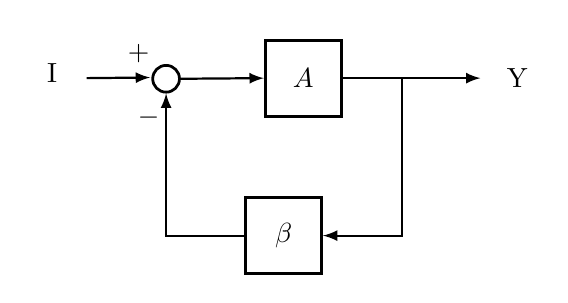
\begin{tikzpicture}[transform shape]
	\node[shape=rectangle, draw, line width=1pt, minimum width=0.965cm, minimum height=0.965cm](N1) at (8.75, 8.5){} node[anchor=center] at (N1.text){$A$};
	\node[shape=rectangle, draw, line width=1pt, minimum width=0.965cm, minimum height=0.965cm](N2) at (8.5, 6.5){} node[anchor=center] at (N2.text){$\beta$};
	\node[shape=circle, draw, line width=1pt, minimum width=0.34cm] at (7.008, 8.492){};
	\draw[line width=0.8pt, -latex] (9.25, 8.5) -- (11, 8.5);
	\draw[line width=0.8pt, -latex] (10, 8.5) |- (9, 6.5);
	\draw[line width=0.8pt, -latex] (8, 6.5) -| (7.008, 8.305);
	\draw[line width=0.8pt, -latex] (7.195, 8.492) -- (8.25, 8.5);
	\draw[line width=0.8pt, -latex] (6, 8.5) -- (6.805, 8.508);
	\node[shape=rectangle, minimum width=0.34cm, minimum height=0.34cm] at (6.625, 8){} node[anchor=center, align=center, text width=-0.048cm, inner sep=6pt] at (6.625, 8){$-$};
	\node[shape=rectangle, minimum width=0.34cm, minimum height=0.34cm] at (6.5, 8.813){} node[anchor=center, align=center, text width=-0.048cm, inner sep=6pt] at (6.5, 8.813){$+$};
	\node[shape=rectangle, minimum width=0.59cm, minimum height=0.59cm] at (5.562, 8.563){} node[anchor=center, align=center, text width=0.202cm, inner sep=6pt] at (5.562, 8.563){I};
	\node[shape=rectangle, minimum width=0.59cm, minimum height=0.59cm] at (11.438, 8.5){} node[anchor=center, align=center, text width=0.202cm, inner sep=6pt] at (11.438, 8.5){Y\\};
\end{tikzpicture}

	\caption{Example of feedback system.}
	\label{ex2}		
	\end{center}	
	\end{figure}
	
\end{enumerate}

As seen in this brief example we can solve the problem of having a small linearity region by implementing a feedback to the negative terminal (inverting input) to reduce, in other words keep under control, the differential voltage by feeding back a part (represented by $\beta$) of the output signal.

In this case we are no longer using an open-loop configuration hence we will talk about closed-loop gain or just gain of the amplifier.
This specific configuration, of feeding back some part of the signal, will be the fundaments of creating different types of amplifier that will serve many different poorhouses.\\

Before moving on we can analyze the reactions between the input and output of the system we created following \autoref{ex2}. Naming $I$ as the input and $Y$ and remembering the operational amplifier relations (writing out the control system block diagram).

We also remember that:

\begin{enumerate}[label=\textbf{-}]
	\item $I$ = Input signal.
	\item $Y$ = Output signal.
	\item $A$ = Open-loop gain of the amplifier.
	\item $\beta$ = feedback factor (fraction of $Y$ returned).
	\item $A\beta$ = Loop gain.
\end{enumerate}

We also have to take into consideration the error generated by the summing node:

\begin{equation}
	e = I - \beta Y
\end{equation}

Since the amplifier gives:

\begin{equation}
	Y = Ae
\end{equation}

Substituting $e$:

\begin{equation}
	Y = A(I - \beta Y)
\end{equation}

At this point we can proceed this way:

\begin{equation}
	Y = A(I - \beta Y) \rightarrow Y = AI - A\beta Y
\end{equation}

Moving $Y$ gets:

\begin{equation}
	Y + A\beta Y = AI
\end{equation}

We can factor out $Y$:

\begin{equation}
	Y(1 + A\beta) = AI
\end{equation}

Solving for $Y$ gets us:

\begin{equation}
	Y = \frac{A}{1 + A\beta} I
\end{equation}

Or if we want to see the relation between input and output we have that identifies the closed-loop gain:

\begin{equation}
	\frac{Y}{I} = \frac{A}{1 + A\beta}
\end{equation}

We can also write this formula this way to make it better to understand:

\begin{equation}
	\frac{Y}{I} = \frac{1}{\beta} \cdot \frac{A \beta }{1 + A\beta} 
\label{solvex}
\end{equation}

At this point since $A \rightarrow \infty$ we can operate on the obtained formula by dividing both numerator and denominator for $A$.

\begin{equation}
	\frac{Y}{I} = \frac{1}{\frac{1}{A} + \beta}
\end{equation}

So we now have $\frac{1}{A} \rightarrow 0$:

\begin{equation}
	\frac{Y}{I} \approx \frac{1}{\beta}
\end{equation}

At this point we can stop and appreciate the idea that gain is no longer determined by the op amp itself, but by the feedback network which is the fundamental idea of negative feedback amplifiers.\\

At this point we can extrapolate a certain value of $\beta$ given the gain that we want to obtain. Since $\beta$ is defined as:

\begin{equation}
	\beta = \frac{R_1}{R_1 + R_2}
\end{equation}

and $\frac{1}{\beta}$:

\begin{equation}
	\frac{1}{\beta} = \frac{R_1 + R_2}{R_1} = 1 + \frac{R_2}{R_1}
\end{equation}

In the end we want to recall that:

\begin{equation}
	\frac{1}{\beta}
\end{equation}

is the ideal gain and that:

\begin{equation}
	\frac{A\beta}{1 + A\beta}
\end{equation}

is the correction factor caused by finite open-loop gain.
Also we remember that:

\begin{equation}
	\frac{A\beta}{1 + A\beta} = \frac{1}{\beta} \cdot \frac{A\beta}{1 + A\beta}
\end{equation}

Especially if $A\beta \gg 1$ then:

\begin{equation}
	\frac{A\beta}{1 + A\beta} \approx 1 \hspace{10pt} \unit{and} \hspace{10pt} G \approx \frac{1}{\beta}
\end{equation}

\paragraph{Example exercise}  Design a voltage amplifier with a gain $G = 3$. Since we are using an ideal op-amp we assume that $A$ is infinite hence the gain will be:

\begin{equation}
	\frac{Y}{I} = \frac{1}{\beta}
\end{equation}

That means we can determine the gain via the formula seen above. We get that:

\begin{equation}
	1 + \frac{R_2}{R_1} = 3 \rightarrow \frac{R_2}{R_1} = 2 \rightarrow R_2 = 2 \cdot R_1
\end{equation}

In this case, since we are still assuming an ideal behavior we can choose any resistor size from the E-series.
We decide that $R_1 = 12$k$\Omega$ $\pm$ 5\%, then $R_2$ should be 24k$\Omega$. Since neither of these values are inside the E-serie we choose one between 27k$\Omega$ or 22k$\Omega$.

We decide to proceed with $R_2 = 22$k$\Omega$ $\pm$ 5\%
We get:

\begin{equation}
	G = 1 + \frac{R_2}{R_1} = 1 + \frac{22}{12} = 2.83
\end{equation}

We can also derive the relative uncertainty on our calculation:

\begin{equation}
	\varepsilon_G = \frac{\Delta G}{G} = \frac{3 - 2.83}{3} = 0.056 = 5.6 \%
\end{equation}

\subsubsection{Voltage follower}

One variation of the circuit we have discussed at length is the one shown in the following \ref{ex6}

\begin{figure}[h!]
\begin{center}

\begin{tikzpicture}[transform shape]
	\node[op amp] at (6.19, 13.49){};
	\draw (4.5, 13) to[european voltage source, v_<=$V_{in}$, voltage/shift=0.3] (4.5, 11.75);
	\draw (4.5, 13) -- (5, 13);
	\node[ground] at (4.5, 11.75){};
	\draw (7.38, 13.49) -| (8, 13.5);
	\node[ocirc](N1) at (8, 13.49){} node[anchor=south] at ([yshift=0.09cm]N1.text){$V_{out}$};
	\node[circ] at (7.38, 13.49){};
	\draw (4.625, 13.98) -| (4.5, 15) -- (7.25, 15) -| (7.375, 13.5);
	\draw (5, 13.98) |- (4.625, 13.98);
\end{tikzpicture}

\caption{Voltage follower}	
\label{ex6}
\end{center}	
\end{figure}


In this topology, the maximum possible feedback is achieved: the fact that the feedback is a short circuit maximizes the portion of the signal fed back to the input ($\beta$ = 1); the consequences are, on the one hand, to make the circuit gain unitary, but on the other hand to make the loop gain as high as possible, greatly increasing the input impedance and reducing the output impedance by the same factor; this circuit will therefore draw very little current from the input, and at the output it will essentially be an ideal voltage generator (i.e., with virtually zero impedance).

The voltage follower configuration is widely used precisely as an \textit{"impedance separator"}. 

We will return to the voltage follower when we discuss the frequency response of operational amplifiers.\\

Given this introduction on the voltage follower we can see that $R_1 = \infty$ and that $R_2 = 0$. This will get us:

\begin{equation}
	G = 1 + \frac{R_2}{R_1} = 1 + \frac{0}{\infty} = 1
\end{equation}

In other terms if the gain is one the output voltage will be the same as the input one:

\begin{equation}
	V_{in} = V_{out}
\end{equation}

At this point the voltage follower might be seen as useless since it does not change the signal provided to it. It is true that the signal is not changed in any way but what changes is the ability to have an ideal infinite input impedance meaning it does not load the source providing the current since it does not draw any of it being able, at the same time, to provide current to a load give its zero output impedance.\\

We can show the difference of using or not using one in the following example.

\begin{figure}[h!]
\begin{center}

\begin{tikzpicture}[transform shape]
	\node[op amp] at (9.44, 8.49){};
	\draw (11.125, 8.5) to[american resistor, l_={$R_L$}, v^<=$V_{out}$, voltage/distance from node=0.4, voltage/bump b=0.8, voltage/shift=2] (11.125, 6.75);
	\draw (6.25, 8) to[american resistor, l={$R_s$}] (8.25, 8);
	\draw (6.25, 6.625) to[european voltage source, v=$V_{in}$] (6.25, 8);
	\node[ground] at (6.25, 6.625){};
	\draw (8.25, 8.98) |- (10.625, 10) |- (10.63, 8.49);
	\draw (10.63, 8.49) -| (11.125, 8.5);
	\node[ground] at (11.125, 6.75){};
	\draw (14.875, 9.25) to[american resistor, l={$R_s$}] (16.875, 9.25);
	\draw (14.875, 7.5) to[european voltage source, v=$V_{in}$] (14.875, 9.25);
	\node[ground] at (14.875, 7.5){};
	\draw (16.875, 9.25) to[american resistor, l_={$R_L$}, v^<=$V'_{out}$, voltage/distance from node=0.4, voltage/bump b=0.8, voltage/shift=2] (16.875, 7.5);
	\node[ground] at (16.875, 7.5){};
\end{tikzpicture}

\caption{Voltage follower use case}
\label{voltfoll}	
\end{center}
\end{figure} 

As we can see on the left there is a voltage follower that will get us, as seen before, a gain $G$ of 1 that means $V_{out} = V_{in}$.
On the right the tension $V'_{out}$ will not be equal to the input but it will be determined by the tension divider, we get that:

\begin{equation}
	V'_{out} = V_{in} \cdot \frac{R_L}{R_S + R_L}
\end{equation}

This will get us a gain $G'$:

\begin{equation}
	G' = \frac{R_L}{R_S + R_L}
\end{equation}


\paragraph{Example exercise} It is now asked to designa a non-inverting amplifier with a gain $G = 10000$ knowing that the open-loop gain $A = 100000$.
As seen before we can use the following relations:

\begin{equation}
	G = 1 + \frac{R_2}{R_1} \rightarrow R_2 = 9999R_1
\end{equation}

This means that:

\begin{equation}
	\beta = \frac{1}{G} = \frac{1}{10000}
\end{equation}

Knowing the $A$ open-loop gain we can calculate $A\beta$:

\begin{equation}
	A\beta = \frac{100000}{10000} = 10
\end{equation}

Using now the \autoref{solvex} we get that:

\begin{equation}
	\frac{A\beta}{1 + A\beta} = \frac{10}{1 + 10} = 0.90909
\end{equation}


\paragraph{Example exercise} Design e non inverting voltage amplifier with a gain $G = \sqrt{2}/2 = 0.707$.

As done before we operate using the formula:

\begin{equation}
	G = 1 + \frac{R_2}{R_1}
\end{equation}

Since:

\begin{equation}
	1 + \frac{R_2}{R_1} \geq 1
\end{equation}

we are not able to create a non inverting amplifier with a gain that is less that 1. To be able to achieve this we would need to use some kind of attenuator or an inverting amplifier.\\



\subsubsection{Transresistance amplifier}


Another circuit topology based on the operational amplifier is shown
in \autoref{ex7}.
The input is current-based, the output is voltage-based; since the ratio between the output and the input is dimensionally a resistance, this topology is called a \textit{"transresistance"} amplifier. Since no current enters the inverting terminal of the device, all the current flows through $R_2$, so the output voltage will be equal to:

\begin{equation}
	v_{out} = -I_RR_2
\end{equation}

\begin{figure}[h]
\begin{center}

\begin{tikzpicture}[transform shape]
	\node[op amp] at (6.19, 13.49){};
	\draw (4.5, 13) -- (5, 13);
	\node[ground] at (4.5, 11.75){};
	\draw (7.38, 13.49) -| (8, 13.5);
	\node[ocirc](N1) at (8, 13.49){} node[anchor=south] at ([yshift=0.09cm]N1.text){$v_{out}$};
	\node[circ] at (7.38, 13.49){};
	\draw (5, 13.98) |- (4.625, 13.98);
	\draw (4.5, 13) -| (4.5, 11.75);
	\node[circ] at (4.5, 13.98){};
	\draw (4.5, 13.98) -| (3, 13.875);
	\draw (3, 13.98) to[european current source, i<_=$I_R$] (3, 11.855);
	\node[ground] at (3, 11.75){};
	\draw (3, 11.75) -| (3, 11.855);
	\draw (4.75, 15.125) to[american resistor, l={$R_2$}] (7.38, 15.125);
	\draw (7.38, 13.49) |- (7.375, 15.125);
	\draw (4.625, 13.98) -- (4.5, 13.98);
	\draw (4.5, 13.98) |- (4.5, 15.125) -- (4.75, 15.125);
\end{tikzpicture}


\label{ex7}
\caption{Transresistance amplifier schematics}	
\end{center}	
\end{figure}


Essentially, this circuit topology \textit{"converts"} current into voltage, providing a voltage output that is proportional to the resistance $R_2$. Upon analyzing this circuit, it is easy to see that both the input and output impedances are very low.

\subsubsection{Inverting amplifier}

The transresistance amplifier forms the basis of this topology, which, together with the non-inverting amplifier, represents one of the most common configurations for the linear operation of the operational amplifier. 

In this case, as we will see shortly, this topology will form the basis of many other linear circuits based on the active device. If, starting from the previous topology, we replace the current source with a voltage source, followed by a series resistor as shown in \autoref{ex7}, we obtain a configuration in which the input voltage is first converted into a current, which is then converted back into voltage at the amplifier’s output.

\begin{figure}
\begin{center}

\begin{tikzpicture}[transform shape]
	\node[op amp] at (6.19, 13.51){};
	\draw (4.5, 13.02) -- (5, 13.02);
	\node[ground] at (4.5, 11.77){};
	\draw (7.38, 13.51) -| (8, 13.52);
	\node[ocirc](N1) at (8, 13.51){} node[anchor=south] at ([yshift=0.09cm]N1.text){$v_{out}$};
	\node[circ] at (7.38, 13.51){};
	\draw (5, 14) |- (4.625, 14);
	\draw (4.5, 13.02) -| (4.5, 11.77);
	\node[circ] at (4.5, 14){};
	\node[ground] at (3, 11.75){};
	\draw (3, 11.75) -| (3, 11.855);
	\draw (4.75, 15.145) to[american resistor, l={$R_2$}] (7.38, 15.145);
	\draw (7.38, 13.51) |- (7.375, 15.145);
	\draw (4.625, 14) -- (4.5, 14);
	\draw (4.5, 14) |- (4.5, 15.145) -- (4.75, 15.145);
	\draw (4.5, 14) to[american resistor, l_={$R_1$}] (3, 14);
	\draw (3, 14) to[european voltage source, v<=$V_i$] (3, 11.875);
\end{tikzpicture}
	
\label{ex8}	
\caption{Inverting amplifier schematics}
\end{center}	
\end{figure}


Before presenting the (brief) calculation of this circuit’s gain, let’s start by pointing out its weakness: the input resistance, $R_i$, is equal to $R_1$, that is, the resistance in series with the input voltage source. 
In fact, since $R_1$ is connected between a voltage source and a \textit{"virtual 0 V"} terminal—that is, a terminal with zero potential difference relative to a terminal connected to 0 V (the non-inverting terminal), we can say that the loop equation toward 0 V via the "$-$" terminal holds; by introducing a test voltage source $V_x$, we will have, across $R_1$ a current $I_x$ equal to:

\begin{equation}
	I_x = \frac{V_x}{R_1} \rightarrow z_1 = \frac{V_x}{I_x} = R_1
\end{equation}


At this point, we know how much current flows through $R_1$, but we also know that no current flows into the op-amp (using the ideal model, which so far has proven to be quite accurate; we may revisit this later); all of the current (already quantified as the ratio of the input voltage to $R_1$) will therefore flow through $R_2$, so that we have:


\begin{equation}
	V_{out} = - \frac{V_{in}}{R_1} \cdot R_2
\end{equation}

From which:

\begin{equation}
	\frac{V_{out}}{V_{in}} = - \frac{R_2}{R_1}
\end{equation}

Therefore, this amplifier, is capable of amplifying (in very simple terms, depending solely on the ratio of the resistors) and inverting the phase (rotating it by 180°) of the input signal. Taking into account the finite gain ($A_d$) of the operational amplifier, we can recalculate to obtain:

\begin{equation}
\frac{V_{in} + v_d}{R_1} = \frac{-v_d - V_{out}}{R_2}
\end{equation}

But since $v_d = V_{out} / A_d$, from which:

\begin{equation}
	V_{in} = -V_{out} \left( \frac{R_1}{R_2} + \frac{R_1 + R_2}{A_dR_2} \right)
\end{equation}

By introducing $\beta$ = $\frac{R_1}{R_1 + R_2}$ and rearranging the terms, we finally obtain:

\begin{equation}
	\frac{V_{out}}{V_{in}} = - \frac{R_2}{R_1} \cdot \frac{1}{1 + \frac{1}{A_d \beta}} = \left( 1 - \frac{1}{\beta} \right) \cdot \frac{1}{1 + \frac{1}{\beta}}
\end{equation}


We have thus obtained another type of amplifier. The problem, however, is that this is not a true voltage amplifier. We have already noted that its input impedance is equal to $R_1$, which is far from high; therefore, its performance is influenced by the output impedance of the signal source, which will reduce the gain of the stage. 
As for the output impedance, it suffices to note that the circuit used for the calculation is the same as in the case of the non-inverting amplifier, so we obtain the same value calculated in \autoref{nonidopamp}.

\subsubsection{Current amplifier}	


\autoref{ex9} shows the schematic of an amplifier whose input is again a current source, $I_s$. 


\begin{figure}
\begin{center}

\begin{tikzpicture}[transform shape]
	\node[op amp, yscale=-1] at (6.19, 14.49){};
	\node[ground] at (4.5, 14.875){};
	\draw (5, 14.98) -| (4.5, 14.875);
	\draw (3, 12) to[european current source, i<^=$I_s$, current/distance=0.2] (3, 14);
	\draw (5, 14) -- (3, 14);
	\node[ground] at (3, 12){};
	\node[circ] at (4.5, 14){};
	\node[circ](N1) at (7.375, 12.25){} node[anchor=west] at ([xshift=0.08cm]N1.text){$A$};
	\draw (7.38, 14.49) to[american resistor, l={$R_L$}, i_=$I_L$, current/distance=0.2] (7.375, 12.25);
	\draw (7.375, 12.25) to[american resistor, l={$R_1$}] (5.75, 12.25);
	\draw (7.38, 12.24) to[american resistor, l={$R_2$}] (7.375, 10.5);
	\draw (5.75, 12.25) -| (4.5, 14);
	\node[ground] at (7.375, 10.5){};
\end{tikzpicture}


\label{ex9}
\caption{Current amplifier}	
\end{center}	
\end{figure}


As in the case of the transresistance amplifier, and whose output is the current $I_L$ in the load resistor $R_L$. 
Considering a real operational amplifier, since the non-inverting input is at 0 V, the inverting input will also be approximately at 0 V (virtual ground). Since no current enters the operational amplifier’s inputs, the current $I_s$ will flow through resistor $R_1$. The voltage at node $A$ will be $V_A$ = $R_1I_s$, and the current $I_{R_2}$ through resistor $R_2$ will be given by:

\begin{equation}
	I_{R_2} = \frac{V_A}{R_2} = I_s \frac{R_1}{R_2}
\end{equation}

At node $A$, we have $I_L + I_s = I_{R_2}$, from which we can obtain:

\begin{equation}
	I_L = I_s \left( 1 + \frac{R_1}{R_2} \right)
\end{equation}

The fact that the input current $I_L$ does not depend on the value of the load resistor $R_L$ means that the circuit’s output behaves like a current source whose value is proportional to the input current. We therefore have a current amplifier with high output impedance and a gain of:

\begin{equation}
	A_I = \left( 1 + \frac{R_1}{R_2} \right)
\end{equation}

Since the input voltage $v_i = -v_d$ is close to 0 V, the input impedance $Z_i = \frac{v_1}{I_s}$ will be very small, ideally infinitesimal. 

A more precise estimation of $Z_i$ can be obtained using the operational amplifier model with differential input impedance and non-infinite gain, as done in the previous sections. The calculations are left as an exercise. % TODO HERE!





\subsubsection{Transconductance amplifier}


The final amplifier variant we will consider in this chapter is shown in \autoref{ex10}. 

\begin{figure}
\begin{center}

\begin{tikzpicture}[transform shape]
	\node[op amp, yscale=-1] at (6.19, 14.51){};
	\node[ground] at (3, 12){};
	\node[circ](N1) at (7.375, 12.25){} node[anchor=west] at ([xshift=0.08cm]N1.text){$A$};
	\draw (7.38, 14.51) to[american resistor, l={$R_L$}, i_=$I_L$, current/distance=0.2] (7.375, 12.27);
	\draw (7.38, 12.24) to[american resistor, l={$R_1$}] (7.375, 10.5);
	\node[ground] at (7.375, 10.5){};
	\draw (3, 12) to[european voltage source, v=$V_{in}$] (3, 14);
	\draw (3, 14) -| (3, 15) -- (4.5, 15);
	\draw (4.5, 15) -- (5, 15);
	\draw (5, 14.02) -| (4.5, 14) |- (7.375, 12.25);
\end{tikzpicture}


\label{ex10}
\caption{Transconductance amplifier}	
\end{center}	
\end{figure}


In this case, the input is a voltage $V_{in}$, and the output is the current $I_L$ flowing through the load resistor $R_L$.

The analysis of this circuit is very simple. Since $v_d \approx 0 V, V_A = V_{in}$, and the current $I_{R_1}$ through resistor $R_1$ is given by $\frac{V_A}{R_1}$. Since no current flows through the inverting input of the op-amp, we have $I_L = I_{R_1}$. We therefore have:

\begin{equation}
	I_L = V_{in} \frac{1}{R_1}
\end{equation}

The proportionality factor between input and output is, in terms of physical units, a conductance, hence the amplifier’s name. In this case, both the input impedance and the output impedance are very high.


\subsubsection{Non-ideal operational amplifiers}
\label{nonidopamp}

Our discussion involves several approximations: real operational amplifiers have characteristics that deviate from the ideal model.

We have seen that a non-inverting amplifier can be constructed simply by selecting the resistors in the feedback loop to achieve a certain gain. But is the gain really the only thing that matters? To put the question another way: does using 1 $\Omega$ and 9 $\Omega$ resistors produce the same result as using 1 M$\Omega$ and 9 M$\Omega$ resistors, or 1 m$\Omega$ and 9 m$\Omega$ resistors? The answer is obviously no: real operational amplifiers exhibit non-ideal effects such that they are affected by the order of magnitude of the resistors used.  As can be seen from a study of the operational amplifier at the transistor level, we will see why it is not possible to use just any resistor. Essentially, the non-idealities are:

\begin{enumerate}[label=\textbf{-}]
	\item The gain $A_d$ is not infinite
	\item Non-infinite differential resistance rd and non-zero output resistance;
	\item Non-zero input currents;
	\item Non-zero differential voltage;
	\item Non-infinite input voltage and output voltage/current dynamics.
\end{enumerate}


Let us proceed step by step, presenting models that are progressively more refined than the ideal one; note that the approach used here does not explain the non-idealities, but rather studies the circuit’s behavior in the presence of a non-ideality. 
The justification for the presence of non-idealities, starting with an examination of the internal workings of the operational amplifier, will be provided later in this discussion.

\subsubsection*{Differential gain}

We present an initial refinement of our model: of the non-idealities listed above, let us consider the fact that $A_d < \infty$. The fact that $A_d$ is not infinite implies that, in order to have a non-zero output, a $v_d \neq 0$ is required. The new model of the device, therefore, will be that shown in figure \ref{ex3}.


\begin{figure}[h]
\begin{center}

\begin{tikzpicture}[scale = 0.75, transform shape]
	\node[ground] at (1, 11){};
	\node[ground] at (3, 7){};
	\node[ground] at (8, 8){};
	\draw (1, 11) to[american resistor, l={$R_1$}] (3, 11);
	\draw (7.125, 15) to[american resistor, l={$R_2$}] (9.125, 15);
	\draw (3, 7) to[european voltage source, v=$v_{in}$] (3, 9);
	\draw (3, 11) -- (5, 11);
	\draw (3, 9) -- (5, 9);
	\node[ocirc] at (5, 11){};
	\node[ocirc] at (5, 9){};
	\draw (5, 11) to[open, v^>=$v_d$, voltage/distance from node=0.8, voltage/bump b=0.2] (5, 9);
	\draw[line width=0.8pt, dash pattern={on 3.2pt off 3.2pt}] (3.75, 14) -| (3.75, 6);
	\draw[line width=0.8pt, dash pattern={on 3.2pt off 3.2pt}] (3.75, 6) -- (12, 10) -- (3.75, 14);
	\draw (8, 10) -- (13, 10);
	\draw (8, 8) to[european controlled voltage source, v^>=$A_dv_d$, voltage/distance from node=1, voltage=straight] (8, 10);
	\draw (3, 11) -| (3, 15) -- (7.125, 15);
	\draw (9.125, 15) -| (12.5, 10);
	\node[circ] at (12.5, 10){};
	\node[circ] at (3, 11){};
	\node[ocirc](N1) at (13, 10){} node[anchor=north] at (N1.text){$v_{out}$};
	\node[shape=rectangle, minimum width=0.59cm, minimum height=0.59cm] at (4.063, 9.313){} node[anchor=center, align=center, text width=0.202cm, inner sep=6pt] at (4.063, 9.313){$+$};
	\node[shape=rectangle, minimum width=0.59cm, minimum height=0.59cm] at (4.125, 11.313){} node[anchor=center, align=center, text width=0.202cm, inner sep=6pt] at (4.125, 11.313){$-$};
\end{tikzpicture}

\caption{First circuit model of the non-ideal operational amplifier: $A_d < \infty$.}
\label{ex3}	
\end{center}	
\end{figure}

We will then have that:

\begin{equation}
	v_- = v_{in} - v_d = v_{out} \cdot \beta
\end{equation}

However, one could also say that:

\begin{equation}
	v_d = \frac{v_{out}}{A_d}
\end{equation}

From here we get that:

\begin{equation}
	v_i - \frac{v_{out}}{A_d} = v_{out} \cdot \beta \rightarrow v_{out} \left( \beta + \frac{1}{A_d} \right)
\end{equation}

Therefore:

\begin{equation}
	v_{out} \cdot \frac{\beta A_d + 1}{A_d} = v_{in} \rightarrow \frac{v_{out}}{v_{in}} = \frac{A_d}{1 + \beta A_d} = \frac{1}{\beta} \cdot \frac{\beta A_d}{1 + \beta A_d} = \frac{1}{\beta} \cdot \frac{T}{1 + T}
\end{equation}


In feedback circuit theory, $T \triangleq \beta A_d $ is the \textit{"loop gain"}. Note, from this model, that in practical cases the deviation of the circuit’s behavior from the ideal case is very small: to achieve a 50\% deviation from the ideal case, the loop gain, $T$ would need to be 1. In reality, even the worst operational amplifiers might have a differential gain, $A_d$ of 10,000; by imposing a very high gain value on the circuit, $\beta$ could be around 1/1000. Few real circuits require a single amplification stage to have such a high gain, because this would cause problems with the circuit’s frequency response. In any case:

\begin{equation}
	T \simeq \frac{10000}{1000} = 10
\end{equation}

Even under these extremely harsh conditions, there is still a 10\% deviation between the gain of the actual circuit and that of the ideal circuit, which is generally acceptable.

\subsubsection*{Input impedance}

We can complicate our discussion by introducing other non-idealities: the impedances of operational amplifiers. Let’s consider a differential resistance $r_d$ that is not infinite (we will not consider the output resistance for now, so the voltage is still taken from an ideal voltage source). We want to calculate this, and to do so, we introduce a known test voltage source, $V_x$, at the input. In order to determine the input impedance, we calculate the current flowing out of $V_x$;

\begin{equation}
	V_x = I_x \cdot r_d + R_1 \cdot (I_{out} + I_x)
\end{equation}

We obtain that:

\begin{equation}
	v_d = r_d \cdot I_x \hspace{1cm} v_{out} = A_dv_d = A_dr_dI_x
\end{equation}

Furthermore:

\begin{equation}
	v_{out} = R_2 I_{out} + R_1(I_{out} + I_x) \rightarrow A_dr_dI_x = R_2I_{out} + R_1(I_{out} + I_x)
\end{equation}

By factoring out the term $I_{out}$:

\begin{equation}
	I_{out}(R_1 + R_2) = A_dr_dI_x - R_1Ix \rightarrow I_{out} = \frac{A_dr_dI_x - R_1I_x}{R_1 + R_2}	
\end{equation}

Substituting this into the expression for $V_x$, we can determine:

\begin{equation}
	V_x = I_xr_d + R_1I_x + \left( \frac{A_dr_dI_x - R_1I_x}{R_1 + R_2} \right) R_1
\end{equation}

From which:

%% TYPO TO FIX I GUESS!

\begin{equation}
	V_x = I_xr_d + \frac{R_1}{R_1 + R_2} A_dr_dI_x + \frac{R_1R_2 + R_1^2 - R_2^2}{R_1 + R_2} I_x
\end{equation}

Recalling that $\beta = \frac{R_1}{R_1 + R_2}$ we obtain that:

\begin{equation}
	z_{in} = \frac{V_x}{I_x} = r_d (1+ \beta A_d) + \beta R_2
\end{equation}

The second term can often be considered negligible compared to the first
(it contributes to increasing the impedance, so neglecting it yields a
\textit{"worst-case"} scenario); what is interesting is that even this model, which is significantly more refined than the ideal one, does not entail any particular changes to the circuit’s behavior: the series-comparison feedback significantly increases the circuit’s input impedance, making the assumption of an ideal operational amplifier acceptable once again in many of our calculations.\\

We end this second case by giving the previous seen model with the addition of the input resistance $r_d$ and by showing the currents $I_{out}$ and $I_x$ (\autoref{ex4}).

\begin{figure}[h]
\begin{center}

\begin{tikzpicture}[scale = 0.75, transform shape]
	\node[ground] at (1, 11){};
	\node[ground] at (3, 7){};
	\node[ground] at (8, 8){};
	\draw (1, 11) to[american resistor, l={$R_1$}] (3, 11);
	\draw (7.125, 15) to[american resistor, l={$R_2$}, i^<=$I_{out}$, current/distance=1] (10.5, 15);
	\draw (3, 7) to[european voltage source, v=$V_{x}$, i^>=$I_x$, current/distance=0.6] (3, 9);
	\draw (3, 11) -- (5, 11);
	\draw (3, 9) -- (5, 9);
	\draw[line width=0.8pt, dash pattern={on 3.2pt off 3.2pt}] (3.75, 14) -| (3.75, 6);
	\draw[line width=0.8pt, dash pattern={on 3.2pt off 3.2pt}] (3.75, 6) -- (12, 10) -- (3.75, 14);
	\draw (8, 10) -- (13, 10);
	\draw (3, 11) -| (3, 15) -- (7.125, 15);
	\draw (10.5, 15) -| (12.5, 10);
	\node[circ] at (12.5, 10){};
	\node[circ] at (3, 11){};
	\node[ocirc](N1) at (13, 10){} node[anchor=north] at (N1.text){$v_{out}$};
	\draw (8, 10) to[european controlled voltage source, v_<=$A_dv_d$] (8, 8);
	\draw (5, 11) to[american resistor, l_={$r_d$}, label distance=0.14cm, v^=$v_d$, voltage/bump b=0.5, voltage/shift=1.6] (5, 9);
	\node[shape=rectangle, minimum width=0.715cm, minimum height=0.715cm] at (4.125, 9.375){} node[anchor=center, align=center, text width=0.327cm, inner sep=6pt] at (4.125, 9.375){$+$};
	\node[shape=rectangle, minimum width=0.715cm, minimum height=0.715cm] at (4.125, 11.375){} node[anchor=center, align=center, text width=0.327cm, inner sep=6pt] at (4.125, 11.375){$-$};
\end{tikzpicture}

\label{ex4}
\caption{Second circuit diagram of the operational amplifier:
input resistor.}
\end{center}
\end{figure}

\subsubsection*{Exit impedance}

In order to refine the model already presented, we must consider the possible effects of the output impedance. Let us therefore consider the operational amplifier model shown in \autoref{ex5}.

To calculate the output impedance, we connect a test voltage generator to it—the usual $V_x$—and thus consider all other independent generators in the circuit to be turned off (the driven ones, of course, are not!). The current $I_x$ will consist of two components: one entering the branch of the driven generator $A_dv_d$ and one entering the branch of $R_2$; we can simplify the analysis by noting that $I_2 \ll I_1$:  since $r_o$ is a much smaller resistance than $R_1$, $R_2$, and even their parallel combination, we could say that $I_x  \simeq I_1$. Neglecting $I_2$ results in a higher impedance value than the actual one, which is acceptable when we want to verify that the output impedance is reasonably low. 

We therefore have that:

\begin{equation}
	I_x \simeq I_1 = \frac{V_x - A_dv_d}{r_o}
\end{equation}

However, we also know that $v_d$ can be expressed as:

\begin{equation}
	v_d = - \beta V_x = -\frac{R_1}{R_1 + R_2} V_x
\end{equation}

We can then say that:


\begin{equation}
		I_x \simeq \frac{V_x + A_d \beta V_x}{r_o}
\end{equation}


From here we get:

\begin{equation}
	\frac{I_x}{V_x} \simeq \frac{1+ \beta A_d}{r_o} \hspace{2cm} \beta A_d = T
\end{equation}

Therefore:

\begin{equation}
	Z_o = \frac{V_x}{I_x} \simeq \frac{r_o}{1 + T}
\end{equation}



Suppose we have a resistance of 100 $\Omega$, which is higher than what is found in most real-world amplifiers; if the loop gain were around 1000, we would reduce the resistance by three orders of magnitude, bringing it down to 100 m$\Omega$! 
We can therefore say that this circuit (non-inverting amplifier) is a good voltage amplifier: high input impedance and low output impedance.

\begin{figure}[h]
\begin{center}

\begin{tikzpicture}[scale = 0.75, transform shape]
	\node[ground] at (1, 11){};
	\node[ground] at (3, 7){};
	\node[ground] at (8, 8){};
	\draw (1, 11) to[american resistor, l={$R_1$}] (3, 11);
	\draw (7.125, 15) to[american resistor, l={$R_2$}, i^<=$I_{2}$, current/distance=1] (10.5, 15);
	\draw (3, 11) -- (5, 11);
	\draw (3, 9) -- (5, 9);
	\draw[line width=0.8pt, dash pattern={on 3.2pt off 3.2pt}] (3.75, 14) -| (3.75, 6);
	\draw[line width=0.8pt, dash pattern={on 3.2pt off 3.2pt}] (3.75, 6) -- (12, 10) -- (3.75, 14);
	\draw (3, 11) -| (3, 15) -- (7.125, 15);
	\draw (10.5, 15) -| (12.5, 10);
	\node[circ] at (12.5, 10){};
	\node[circ] at (3, 11){};
	\draw (8, 10) to[european controlled voltage source, v_<=$A_dv_d$] (8, 8);
	\draw (5, 11) to[american resistor, l_={$r_d$}, label distance=0.14cm, v^=$v_d$, voltage/bump b=0.5, voltage/shift=1.6] (5, 9);
	\node[shape=rectangle, minimum width=0.715cm, minimum height=0.715cm] at (4.125, 9.375){} node[anchor=center, align=center, text width=0.327cm, inner sep=6pt] at (4.125, 9.375){$+$};
	\node[shape=rectangle, minimum width=0.715cm, minimum height=0.715cm] at (4.125, 11.375){} node[anchor=center, align=center, text width=0.327cm, inner sep=6pt] at (4.125, 11.375){$-$};
	\draw (3, 7) -| (3, 9);
	\draw (8, 10) to[american resistor, l={$r_o$}, i^<=$I_1$, current/distance=1] (10, 10);
	\draw (10, 10) -- (13, 10);
	\draw (13, 10) to[european voltage source, v<=$V_x$, i=$I_x$] (13, 8);
	\node[ground] at (13, 8){};
\end{tikzpicture}

\caption{Operational amplifier model with non-zero output impedance.}
\label{ex5}	
\end{center}	
\end{figure}



%\subsection{Current Mirrors}
%\subsubsection{BJT Current Mirror}
%\subsection{MOSFET Current Mirror}
%\subsection{BJT Differential Stage}
%
%\subsection{Differential stage}
%\subsubsection{Differential mode and common-mode}
%\subsubsection{BJT differential stage}
%\subsubsection{MOSFET differential stage}
%
%\subsection{Simplified schematic of an operational amplifier}
%
%\subsection{Bipolar transistor power stages}
%\subsubsection{Bipolar power transistors}
%\subsubsection{Power classes}
%\subsubsection{Class A}
%\subsubsection{Class B}
%\subsubsection{Class AB}
%\subsubsection{Design Example}
%
%\subsection{Real operational amplifier models}
%\subsubsection{Voltage and current offset}
%\subsubsection{Common-mode input dynamics}
%\subsubsection{Output dynamics}
%\subsubsection{Input impedances}
%\subsubsection{Differential gain}
%\subsubsection{CMOS operational amplifier}
%
%\subsection{Amplifier sizing}
%\subsubsection{Specifications}
%\subsubsection{Project}
%
%\subsection{Frequency response}
%\subsubsection{Transfer function}
%\subsubsection{Loop gain}
%\subsubsection{Bandwidth-gain product}
%\subsubsection{Slew rate}









\end{document}